\documentclass[french, 11pt, a4paper]{article}

%%%%% PACKAGES %%%%%
\usepackage[utf8]{inputenc}
\usepackage[T1]{fontenc}
\usepackage[french]{babel}
\usepackage[margin=2cm]{geometry}
\usepackage{setspace}
\usepackage{graphicx}
\usepackage{rotating}
\usepackage{url}
\usepackage{float}
\usepackage{listings}
\usepackage{wrapfig}
\usepackage[bottom]{footmisc}
\usepackage{enumitem}
\usepackage{tikz}
\usepackage[colorlinks,allcolors=blue, hidelinks]{hyperref}
\def\checkmark{\tikz\fill[scale=0.4](0,.35) -- (.25,0) -- (1,.7) -- (.25,.15) -- cycle;} 
\newcommand{\subsubsubsection}[1]{\paragraph{#1}\mbox{}\\}
\setcounter{secnumdepth}{4}
\newcommand{\subsubsubsubsection}[1]{\paragraph{#1}\mbox{}\\}
\setcounter{secnumdepth}{6}
\setcounter{tocdepth}{6}
\newcommand{\newpara}{\vskip 0.75cm}
\newcommand{\newparasm}{\vskip 0.2cm}
\newlist{todolist}{itemize}{2}
\setlist[todolist]{label=$\square$}
\usepackage{pifont}
\usepackage{enumitem,amssymb}
\newcommand{\cmark}{\ding{51}}%
\newcommand{\xmark}{\ding{55}}%
\newcommand{\done}{\rlap{$\square$}{\raisebox{2pt}{\large\hspace{1pt}\cmark}}%
\hspace{-2.5pt}}
\newcommand{\wontfix}{\rlap{$\square$}{\large\hspace{1pt}\xmark}}


\begin{document}
\singlespacing

%%%%% PAGE DE GARDE %%%%%

\begin{titlepage}
\begin{center}


\includegraphics[width=15cm]{img/ephec.jpg}~\\
\textsc{Avenue du Ciseau, 15 \\ 1348 Ottignies-Louvain-la-Neuve} \\[1.5cm]

{\huge \bfseries \begin{spacing}{1.25}
  Dévéloppement d'un progiciel \\ 
  de gestion intégré \\
  pour l'entreprise Master Services
  \\[2cm]
  \end{spacing} 
} 

{\large 
  Travail de fin d’études présenté en vue de l’obtention du diplôme de bachelier en Informatique et Systèmes \\
  orientation Technologie de l’Informatique
  \\[2cm]
}

{\LARGE 
JAUJATE OULDKHALA Ikram
}

\vspace*{\fill}
  
\end{center}

\begin{minipage}[t]{.5\textwidth}
  \textsc{\large Rapporteur:\\Monsieur S. Buys}
\end{minipage}
\begin{minipage}[br]{.5\textwidth}
  \textsc{\large Année académique 2021-2022}
\end{minipage}  

\end{titlepage}



%%%%% TOC %%%%%
\singlespacing
\newpage
\addtocontents{toc}{\protect\setcounter{tocdepth}{4}}
\renewcommand{\contentsname}{Table des matières}
\tableofcontents
%%%%% CONTENU %%%%%
\onehalfspacing

\newpage
\section{Introduction}
\subsection{Contexte général }
\subsubsection{Client}

Le client, une entreprise active dans le secteur du bâtimentdes travaux publics, situé à Sint-Pieters-Leeuw doit constamment gérer, dans le cadre de ses activités, le flux de matériaux, ses clients, ses employés, ses fournisseurs ainsi que toutes les facturations qui en découlent.

Il ne possède actuellement aucun moyen informatisé lui permettant de gérer l'ensemble de ses entités. Il m'a été demandé de de concevoir une solution pour répondre à l'ensemble de ses besoins :

\begin{itemize}
  \item Gestion clients 
  \item Gestion des Projets
  \item Gestion Matériel
  \item Gestion Stock
  \item Gestion Main d'Oeuvre
  \item Gestion du personnel
  \item Gestion utilisateurs
  \item Gestion Factures
  \item Gestion Devis

\end{itemize}

\subsection{Objectifs }

Il a donc été décidé, en accord avec le client, que la solution sera déployée de telle sorte qu'elle puisse être adaptée au fil des années en fonction de l'évolution des besoins du client. 
De plus, le client étant souvent sur chantier, il est primordial que l'application puisse être facilement portable d'un système / ordinateur à un autre. Il a donc été décidé en commun accord avec le client que la solution sera déployée sous forme d'une application web ce qui apportera une grande flexibilité au niveau de l'utilisation de la solution.

Le volume d'information à gérer étant conséquent, la visualisation doit principalement être adaptée \textbf{aux écrans d'ordinateur.}

\subsection{Cadre didactique de la réalisation}

Je pense que ce projet rentre tout à fait dans le cadre d'un TFE étant donné qu'il require l'analyse, le développement, le déploiement et la maintenance d'une application web afin d'apporter une solution adéquate répondant aux spécificités d'un client.
Le développement se fera à l'aide de technologies modernes qui me permettront d'offrir une interface au goût du jour et modulable. Afin d'améliorer la productivité, je ferais usage de multiples techniques DevOps telles que le déploiement continu et bien d'autres.




\newpage
\section{Méthode de travail}

\subsection{Méthodologie}

Vu l'envergure du projet et des tâches techniques à accomplir, l'approche sélectionnée pour la réalisation de ce projet est une organisation en mode Agile.
Plus spécifiquement, j'ai décidé de travailler avec le cadre de travail Scrum et son organisation en sprints.

Tout d'abord, j'ai pu définir avec le client les principales fonctionnalités à intégrer dans le projet. Ces fonctionnalités sont classées par ordre de priorité et par temps estimé à la réalisation de celles-ci.

En outre, les principales fonctionnalités contenues dans le projet sont détaillées. S'agissant d'un projet de grande envergure, chacune des principales fonctionnalités a été divisée en petites user stories qui me permettront d'avoir un produit livrable au client à la fin de chaque sprint. Les sprints auront \textbf{une durée d’environ 2 semaines.}

À la fin de chaque sprint, un délivrable correspondant aux tâches / user stories effectuées lors du sprint devra être présenté au client. Ce dernier devra alors vérifier et valider les différentes tâches effectuées.

L'avantage de cette organisation est que, en cas d'erreurs et/ou non validation des tâches de la part du client, ces dernières pourront être revues et corrigées pour le prochain sprint.

\begin{figure}[H]
  \centering
  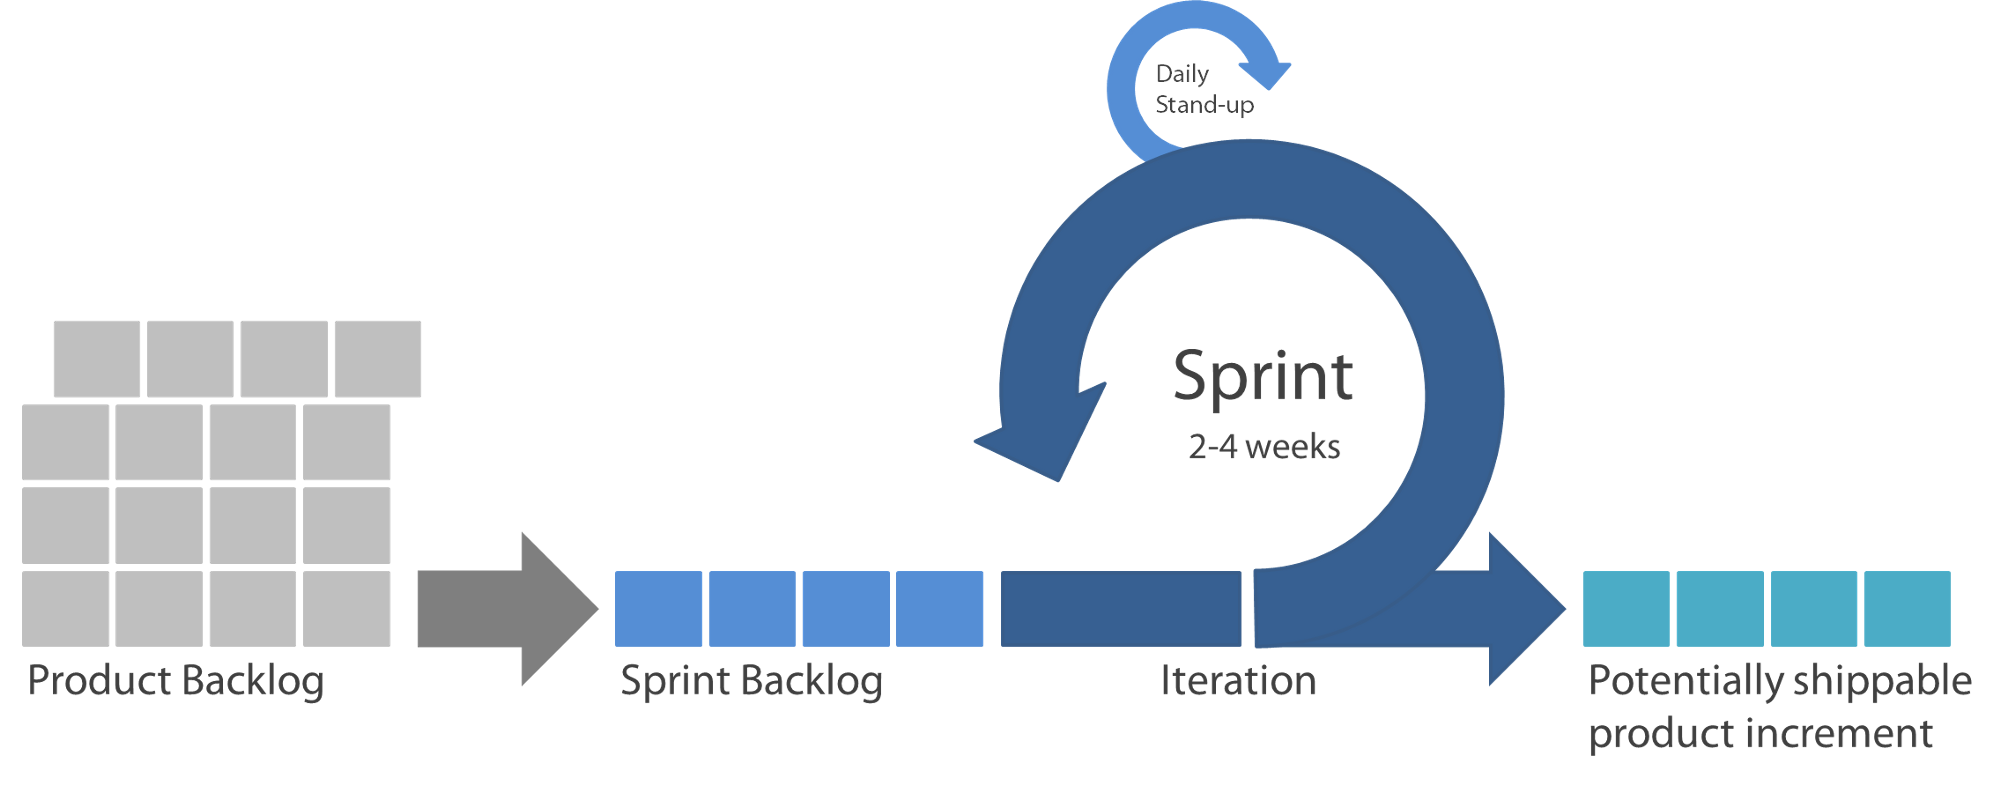
\includegraphics[width=0.75\linewidth]{img/agile.png}
  \caption{ \textit{Cadre de travail Scrum} de Anna Pérez}
  \label{agile}
\end{figure}

\subsubsection{Outils}
Afin d'optimiser les tâches à effectuer pour chaque sprint et d'améliorer ma performance de travail, plusieurs outils ont été utilisés dans l'objectif de faciliter la visualisation de l’avancement du projet.
\begin{itemize}
  \item \textbf{Trello}: Tableau permettant d'organiser les différentes tâches et user stories de manière optimale.
  \item \textbf{Clockify}: Outil de suivi des heures travaillées sur le projet.
  \item \textbf{SqlDBM}: Outil permettant la création de mon schéma de base de données.
\end{itemize}

\subsubsection{Gitflow}

J'ai décidé de travailler avec le gitflow par branche, ce qui permet d'avoir une division au niveau des fonctionnalités qui seront implémentées lors du projet.

\begin{itemize}
  \item Une branche 'develop' qui correspond à la branche 'master' du 'github-flow'
  \item Chaque fonctionnalité est dévéloppée sur une branche spécifique et une fois celle-ci est validée par le client, alors elle est fusionnée avec la branche develop.
\end{itemize}

\begin{figure}[H]
  \centering
  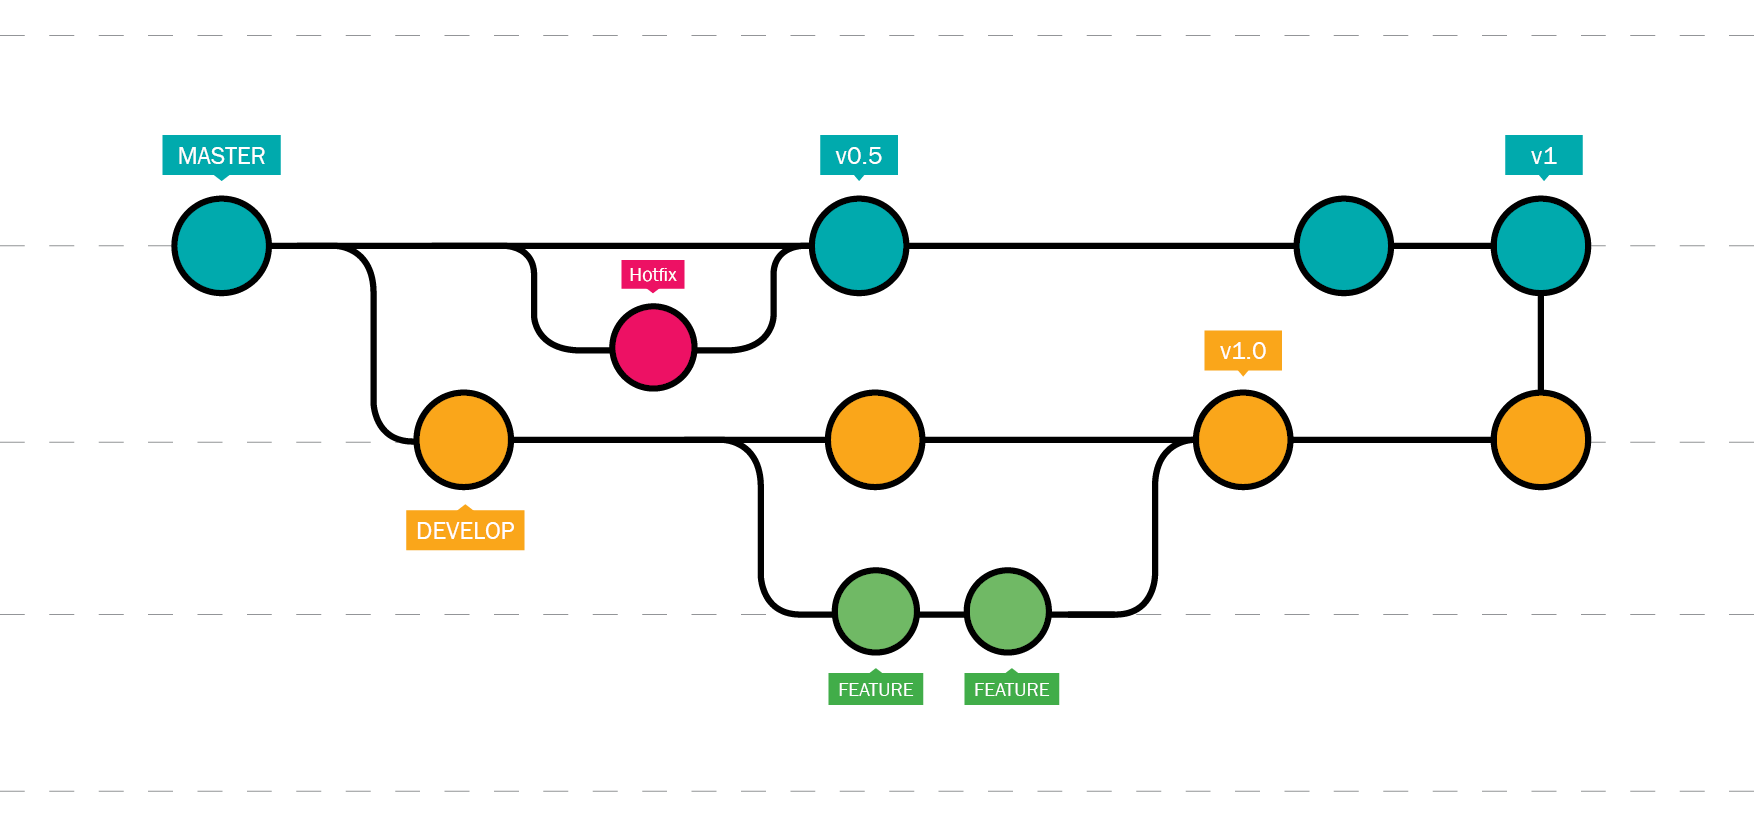
\includegraphics[width=0.75\linewidth]{img/gitflow.png}
  \caption{ \textit{Gitflow Strategy} de Atlassian}
  \label{Gitflow}
\end{figure}


\subsection{Choix des technologies}

\subsubsection{Frontend}
\begin{figure}[H]
  \begin{minipage}{.3\textwidth}
    
\includegraphics[width=0.75\linewidth]{img/react.png}
  \end{minipage}
  \begin{minipage}{.7\textwidth}
    
    En ce qui concerne la technologie frontend, React permet de créer des interfaces utilisateur ou des composants d'interface utilisateur rapides et interactifs pour les utilisateurs d'applications web et mobiles.
    \begin{enumerate}
      \item \textbf{DOM Virtuel}: Il permet de générer le DOM ("Document Object Model", structure des éléments qui sont générés dans le navigateur web lors du chargement d'une page) de manière dynamique, ce qui nous permet de visualiser les changements de données sans devoir recharger à nouveau la page entière, mais seulement le composant qui a été mis à jour.
      \item \textbf{Grande communauté}: Il est soutenu par une large communauté, ce qui nous permet d'avoir un grand nombre de libraires disponibles.
      \item \textbf{Composants réutilisables}: React est constitué de composants qui sont réutilisables, ce qui rend l'application plus portable et plus facile à maintenir.
    \end{enumerate}
    Ces avantages permettent d'améliorer l'expérience de l'utilisateur lors de la navigation dans l'application web, la rapidité du chargement des pages et facilitent la maintenance de l'application.
  \end{minipage}
\end{figure}

\subsubsection{Web Server}

\begin{figure}[H]
  \begin{minipage}{.3\textwidth}
    
\includegraphics[width=0.75\linewidth]{img/caddy.png} 
  \end{minipage} 
  \begin{minipage}{.7\textwidth}
    Au niveau du serveur web, mon choix se porte sur Caddy Server et ce pour plusieurs raisons
    \begin{enumerate}
      \item \textbf{Simple}: Possède une configuration très simple qui nous permettra de le mettre en place en quelques minutes.
      \item \textbf{HTTPS par défaut}: Utilise Let's Encrypt pour mettre le site en HTTPS complet automatiquement, sans aucune configuration et le renouvellement des certificats SSL/TLS se réalise de manière automatique.
      \item \textbf{Multiplateforme}: Il est multiplateforme et je serai en mesure d'exécuter Caddy directement par le biais de Docker, ce qui rendra sa mise en œuvre encore plus facile.
    \end{enumerate}
  \end{minipage} 
\end{figure}

\subsubsection{Backend}
\begin{figure}[H]
  \begin{minipage}{.3\textwidth}
    
\includegraphics[width=0.75\linewidth]{img/node.png} 
  \end{minipage}
  \begin{minipage}{.7\textwidth}

    Comme pour le frontend, le choix du backend est également essentiel. Dans ce cas, j'ai décidé de travailler avec Node.js et ce pour plusieurs raisons.
    \begin{enumerate}
      \item \textbf{Très rapide}: Les tâches courantes comme la lecture ou l’écriture dans la base de données sont exécutées rapidement et il capables de gérer des connexions simultanées à haut débit.
      \item \textbf{Grande communauté}: Il est soutenu par une large communauté, ce qui nous permet d'avoir un grand nombre de libraires disponibles.
      \item \textbf{MVC}: Permet de travailler en MVC, ce qui permet une structure correcte du code.
      \item \textbf{Asynchrone}: Étant un système asynchrone, il permet d’accélérer les applications web. Il est capable d'envoyer gros volumes de données sans bloquer le serveur qui reste ainsi disponible pour traiter d’autres tâches.
      \item \textbf{compatible}: Permet un développement multiplateforme qui est axé sur tous les types d'appareils et de plateformes d'OS (iOS, Android, desktop et web). Le code est réutilisable et entièrement compatible avec tous les principaux systèmes d'exploitation, notamment Linux, Windows, ainsi que macOS, ce qui va nous permettre de rendre notre Web Application accessible depuis toutes les plateformes.
    \end{enumerate}

  \end{minipage}
\end{figure}

\subsubsection{Database}

\begin{figure}[H]
  \begin{minipage}{.3\textwidth}
    
\includegraphics[width=0.75\linewidth]{img/PostgreSql.png} 
  \end{minipage} 
  \begin{minipage}{.7\textwidth}
    Mon choix pour la base de données est PostgreSQL pour plusieurs raisons :
    \begin{enumerate}
      \item \textbf{DB Relationnelle}: Puisque les données doivent être ordonnées et structurées et que des relations doivent exister entre les différentes données, il est essentiel d'utiliser une base de données SQL afin de garantir l'organisation de ces dernières.
      \item \textbf{SQL}: PostgreSQL utilise le langage SQL, qui est le langage le plus utilisé pour les bases de données relationnelles.
      \item \textbf{Compatible}: PostgreSQL est entièrement compatible ACID. ACID est un acronyme pour Atomicité, Cohérence, Isolation et Durabilité. Il garantit donc que les transactions n'interfèrent pas entre elles. Cela garantit les informations contenues dans les bases de données et la pérennité des données dans le système.
      \item \textbf{Hot-Standby}: Il dispose de l'option Hot-Standby qui permet aux utilisateurs d'accéder aux tables en mode lecture pendant que les processus de sauvegarde ou de maintenance sont en cours.

    \end{enumerate}
    PostgreSQL jouit d'une solide réputation en matière de fiabilité, de robustesse des fonctionnalités et des performances.
  \end{minipage} 
\end{figure}


  
\subsection{Autres}
\subsubsection{Documentation API}


L'API (\textit{Application Programming Interfaces}) est le backbone\footnote{\textit{Élement structurelle indispendsable au bon fonctionnement de l'application. Ceci répresente le coeur de l'application.}} d'une application. Elle permet l'interaction d'un utilisateur ou d'une application avec le système d'information sur base d'endpoints.
Pour pouvoir utiliser l'API de manière efficace, il est nécessaire d'avoir une bonne documentation. Cette documentation doit pouvoir exprimé de manière claire l'action de chaque endpoint sur le système d'information. Dès lors on y retrouvera les méthodes telles que GET, CREATE, UPDATE, DELETE, les informations rélatives aux données nécessaires pour le bon déroulement de la requête ainsi qu'un exemple et/ou le format du résultat attendu.
\newpage
Pour pouvoir réaliser cette documentation, il existe un grand nombre de technologies qui permettent de la créer et de la générer automatiquement. Dans mon cas, j'ai décidé d'utiliser \textbf{Swagger}. Celui-ci s'intègre parfaitement avec NodeJS / ExpressJS, il permet d'autogénerer en grande partie la documentation sur base de mes endpoints et il est open-source.
La documentation générée par Swagger est facile à comprendre et permet de tester directement l'API sans devoir passée par un outil supplémentaire tel que Postman.

\begin{figure}[H]
  \centering
  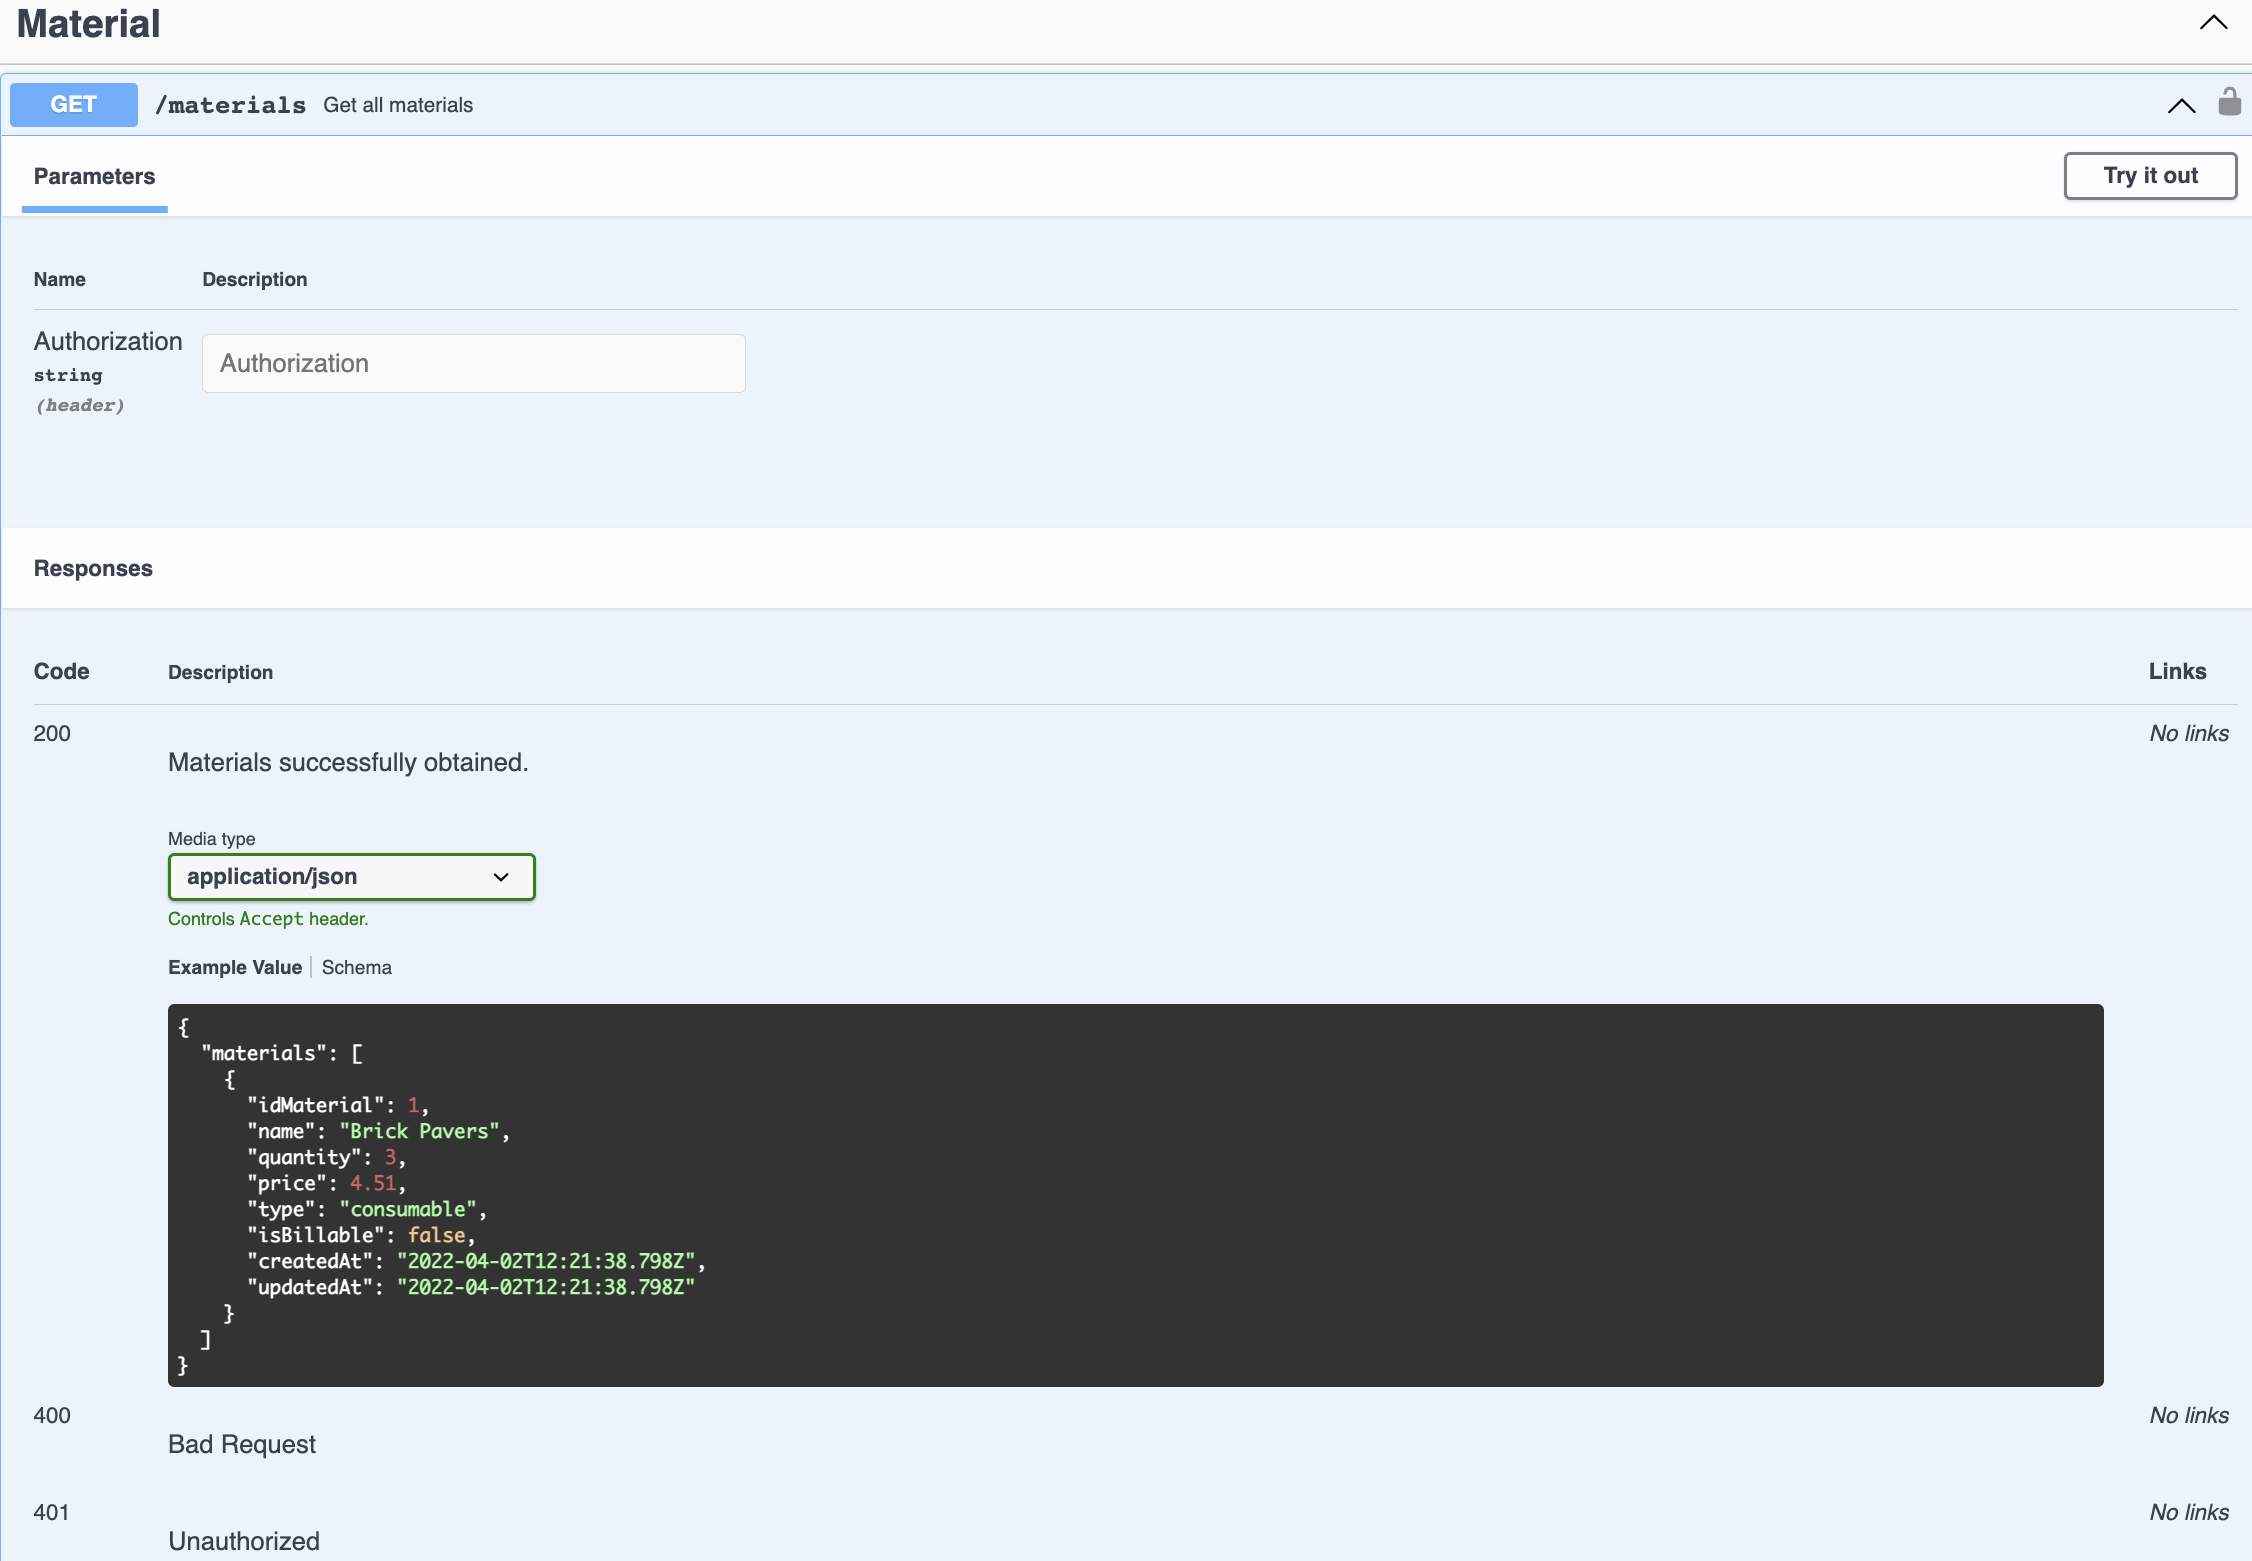
\includegraphics[width=0.75\linewidth]{img/docApi.png}
  \caption{ Documentation API avec Swagger}
  \label{Swagger}
\end{figure}
\subsubsection{Linter}
Dans tout projet, il est inévitable d'avoir des erreurs de syntaxe, des styles de code et bien d'autres problèmes. De plus, avoir un code parfaitement cohérent et lisible est très compliqué. C'est pourquoi l'une des solutions est l'utilisation d'un Linter. Cet outil effectue un check du code source de l'application sans jamais l'exécuter.

Une fois la révision terminée, le Linter nous montre les erreurs de syntaxe, corrige automatiquement l'indentation si cette option a été configurée et fait également des suggestions visant à améliorer le code.

Considérant que c'est une partie essentielle de mon projet, j'ai décidé d'utiliser le Linter et plus précisément ESLint.



\newpage
\section{User Stories}
\subsection{Description }
\subsubsection{Exemple }
\subsection{Liste des fonctionnalités dévélopées}
Toutes les fonctionnalités prévues pour le projet ont été réalisées. 
Ci-dessous, vous pouvez voir une vue non-détaillée des fonctionnalités implémentées.

\textbf{Utilisateur}
\begin{todolist}
    \item[\done] U01 - Connexion utilisateur
    \item[\done] U02 - Consulter les utilisateurs
    \item[\done] U03 - Ajouter un nouveau utilisateur
    \item[\done] U04 - Modifier utilisateur
    \item[\done] U05 - Supprimer utilisateur 
\end{todolist}

\textbf{Clients}
\begin{todolist}
    \item[\done] CLI-1 : Consultation la listes des clients
    \item[\done] CLI-2 : Consulter le détail d’un client
    \item[\done] CLI-3 : Ajouter un nouveau client
    \item[\done] CLI-4 : Modification d'un client
    \item[\done] CLI-5 : Supprimer un client
    \item[\done] CLI-6 : Rechercher un client
    \item[\done] CLI-7 : Trier la liste des clients 
\end{todolist}

\textbf{Projets}
\begin{todolist}
    \item[\done] PRJ-1 : Consulter la listes des projets
    \item[\done] PRJ-2 : Consulter le détail d’un projet
    \item[\done] PRJ-3 : Rechercher un projet
    \item[\done] PRJ-4 : Filtrer un projet
    \item[\done] PRJ-5 : Ajouter d’un projet
    \item[\done] PRJ-6 : Modifier le contenu d’un projet
    \item[\done] PRJ-7 : Supprimer un projet

\end{todolist}

\textbf{Matériel}
\begin{todolist}
    \item[\done] MA-1 : Consulter la liste de matériel disponible
    \item[\done] MA-2 : Consulter le détail d’un matériel
    \item[\done] MA-3 : Ajouter d'un matériel à un projet
    \item[\done] MA-4 : Rechercher d'un matériel 
    \item[\done] MA-5 : Désaffecter un matériau d'un projet
    \item[\done] MA-6 : Modifier un matériel
    \item[\done] MA-7 : Supprimer du matériel

\end{todolist}

\textbf{Devis}
\begin{todolist}
    \item[\done] DE-1 : Consultation devis
    \item[\done] DE-2 : Générer un devis
    \item[\done] DE-3 : Consulter le détail d'un devis 
    \item[\done] DE-4 : Consulter les devis appartenant à un projet
    \item[\done] DE-5 : Envoyer devis par mail
    \item[\done] DE-6 : Recherche un devis
    \item[\done] DE-7 : Trier la liste des devis
\end{todolist}

\textbf{Factures}
\begin{todolist}
    \item[\done] FA-1 : Consultation facture
    \item[\done] FA-2 : Générer une facture
    \item[\done] FA-3 : Consulter détail d'une facture
    \item[\done] FA-4 : Consulter les factures appartenant à un projet
    \item[\done] FA-5 : Envoyer une facture par mail
    \item[\done] FA-6 : Télécharger facture
    \item[\done] FA-7 : Recherche une facture
    \item[\done] FA-8 : Trier la liste des factures

\end{todolist}

\newpage
\input{sections/developpement.tex}

\newpage
\section{Déploiement}
\subsection{Études des différentes solutions}
\subsubsection{Heroku}
\subsubsection{Serveurs dédiés OVH}
\subsection{Justification du choix}
\subsubsection{Docker}
\subsection{Scripts}
\subsection{Intégration et Déploiement Continu}

\newpage
\section{Testing}
\subsection{ Unitaires}
\subsection{ Integrations}
\subsection{ End-to-End}

\newpage
\section{Optimisation}
\subsection{Caching}
\subsubsection{Redis}
\begin{figure}[H]
    \begin{minipage}{.3\textwidth}
      
\includegraphics[width=1\linewidth]{img/redis.png}
    \end{minipage}
    \begin{minipage}{.7\textwidth}
Redis est une base de données NoSQL mais elle n'est pas très similaire aux autres bases de données NoSQL. Cela est dû au fait que Redis ne fonctionne pas vraiment avec des tables, mais toutes les données dans Redis sont stockées dans des paires clé-valeur. 
Il y a donc une clé ayant un nom et une valeur appelée Kyle, ce qui rend Redis similaire à un objet json géant
L'objectif n'est pas de stocker un ensemble de données structurées, mais simplement de stocker une paire clé-valeur individuelle à partir de laquelle nous pouvons accéder aux données.
Il est important de noter que Redis fonctionne en utilisant la mémoire RAM de la machine sur laquelle il tourne. Cela signifie qu'il est extrêmement rapide.
\newpara
Dans le cas où nous devons accéder à des informations qui prennent beaucoup de temps à charger, par exemple une quantité de données assez importante provenant de la base de données, nous pouvons utiliser Redis pour stocker ces valeurs pendant une durée définie. Ainsi, lorsque nous devrons accéder à cette même information, la réponse sera beaucoup plus rapide puisque l'information sera déjà chargée.
\end{minipage}
\end{figure}
\subsubsection{Analyse des résultats}
Le temps de chargement des données sur certaines de mes API était assez important et je devais trouver une solution pour le réduire. 
Afin d'améliorer le temps de chargement des données, j'ai décidé d'utiliser Redis. 
Pour tester Redis, j'ai décidé de récuperer tous les clients se trouvant dans ma base de données, ce qui correspond à, environ, 1400 clients.

\subsubsubsection{Sans utilisation de Redis}
Dans la figure ci-dessous, nous pouvons voir que le temps de réponse de la requête réalisée sans Redis a tendance à diminuer un peu après la première requête. Ceci est dû à la gestion du cache de Sequelize et de Postgres. Bien que ce temps ait diminué, la moyenne de ces temps est encore élevée, elle correspond à 495 ms, une demi-seconde.
\begin{figure}[H]
    \centering
    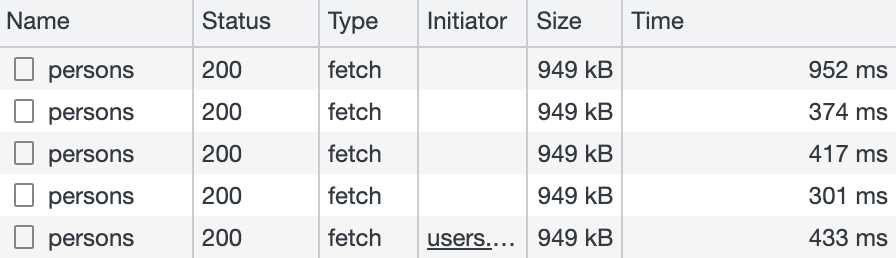
\includegraphics[width=\linewidth]{img/sans-redis.png}
    \caption{Temps de réponse sans Redis}
    \label{Sans-Redis}
  \end{figure}
\subsubsubsection{Avec utilisation de Redis}
La même requête a été faite mais cette fois avec Redis. Dans la figure 5, la première requête, sans Redis, dure une seconde, ce qui est assez conséquant. Les requêtes suivantes utilisant Redis diminuent considérablement en obtenant une moyenne de 204ms.
\begin{figure}[H]
    \centering
    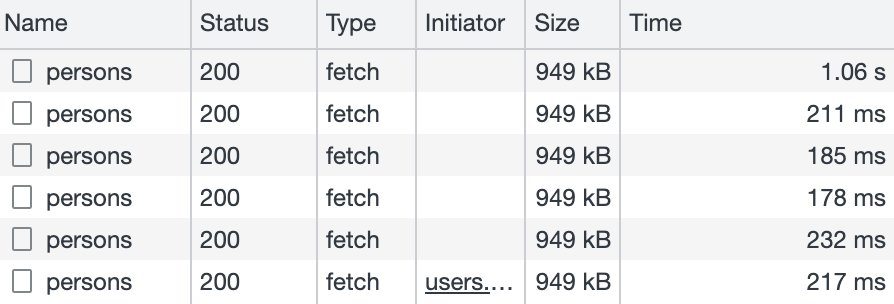
\includegraphics[width=\linewidth]{img/avec-redis.png}
    \caption{Temps de réponse avec Redis}
    \label{Avec-Redis}
\end{figure}
La performance obtenue en utilisant redis a augmenté d'un 58,8\%.



\newpage
\section{Sécurité}
\subsection{Frontend}
\subsubsection{Routage}
\subsection{Backend}
\subsubsection{Routage API}
\subsubsection{Base de données}
\subsubsection{En-têtes HTTPS}

\subsection{Web Server}
\subsubsection{SSH}
\subsubsection{Firewall}
\subsubsection{Reverse-proxy}

\subsection{Autres}
\subsubsection{Libraries}



\newpage
\section{Monitoring}

\newpage
\section{Conclusion}

\newpage
\section{Bibliographie}

\renewcommand{\section}[2]{}%
\begin{thebibliography}{}


\bibitem{React}
Smashing Magazine (2020, 2 mai), sur le site \textit{Implementing Dark Mode In React Apps Using styled-components} Consulté le 20 janvier 2022
\\\url{https://www.smashingmagazine.com/2020/04/dark-mode-react-apps-styled-components/}

\bibitem{User-Story}
Atlassian (2021, 22 mars), sur le site \textit{Beautiful and accessible drag and drop for lists with React} Consulté le 22 janvier 2022
\\\url{ https://github.com/atlassian/react-beautiful-dnd}

\bibitem{User-Story}
User Story (2019), sur le site \textit{User story - Wikipedia} Consulté le 24 novembre 2021
\\\url{https://en.wikipedia.org/wiki/User_story}

\bibitem{Node Js}
Stack Overflow (2020, 10 décembre), sur le site \textit{Upgrading Node.js to latest version} Consulté le 22 décembre 2021
\\\url{https://stackoverflow.com/questions/10075990/upgrading-node-js-to-latest-version}

\bibitem{Node Js}
Tang, R. (2020, 10 décembre), sur le site \textit{How to install Node JS and NPM } Consulté le 14 décembre 2021
\\\url{https://www.makersupplies.sg/blogs/tutorials/how-to-install-node-js-and-npm-on-the-raspberry-pi}

\bibitem{CI-CD}
Terzi, R(2018, 16 novembre), sur le site \textit{Qu'est-ce que l'approche CI/CD ?} Consulté le 22 janvier 2022
\\\url{https://www.redhat.com/fr/topics/devops/what-is-ci-cd}

\bibitem{Agile}
Shadow-M-P (14 mai 2021), sur le site \textit{Méthode agile — Wikipédia} Consulté le 23 janvier 2022
\\\url{https://fr.wikipedia.org/wiki/Méthode_agile}

\bibitem{PostgreSQL}
PostgreSQL Tutorial (sans date), sur le site \textit{PostgreSQL Transactions} Consulté le 3 décembre 2021
\\\url{https://www.postgresqltutorial.com/postgresql-transaction/}

\bibitem{CSP}
PostgreSQL Tutorial (sans date), sur le site \textit{PL/pgSQL For Loop} Consulté le 14 décembre 2021
\\\url{https://www.postgresqltutorial.com/plpgsql-for-loop/}

\bibitem{X-Frame}
PostgreSQL Tutorial (22 mai 2021), sur le site \textit{PostgreSQL CREATE PROCEDURE} Consulté le 3 janvier 2022
\\\url{https://developer.mozilla.org/fr/docs/Web/HTTP/Headers/X-Frame-Options}

\bibitem{X-Content}
Großgarten, G. (2021, 21 janvier), sur le site \textit{Copy a folder to a remote server using SSH} Consulté le 10 novembre 2021
\\\url{https://github.com/garygrossgarten/github-action-scp}

\bibitem{VPS}
OVH (sans date), sur le site \textit{Qu'est-ce qu'un VPS ? Découvrez les avantages d'un VPS | OVHcloud} Consulté le 25 novembre 2021
\\\url{https://www.ovhcloud.com/fr/vps/definition/#:~:text=Grâce%20au%20VPS%2C%20vous%20profitez,en%20payant%20le%20juste%20prix.}

\bibitem{Node Js}
Adaobi, A. (2021, 27 octobre), sur le site \textit{Making HTTP Requests in Node.js with node-fetch} Consulté le 25 novembre 2021
\\\url{https://stackabuse.com/making-http-requests-in-node-js-with-node-fetch/}

\bibitem{conteneurisation}
Laurent Hercé (2020, septembre 15), sur le site \textit{Conteneurisation informatique : définition, avantages, différence virtualisation, solutions | Appvizer} Consulté le 26 décembre 2021
\\\url{https://www.appvizer.fr/magazine/services-informatiques/virtualisation/conteneurisation-informatique}

\bibitem{PostgreSQL}
Stack Overflow (2011, 3 juillet), sur le site \textit{Can I use return value of INSERT. . . RETURNING in another INSERT? } Consulté le 26 décembre 2021
\\\url{https://stackoverflow.com/questions/6560447/can-i-use-return-value-of-insert-returning-in-another-insert}




\end{thebibliography}





\end{document}